\documentclass[a4paper,10pt]{article}
% Use ctrl + alt + V to view live pdf

% Packages
\usepackage[utf8]{inputenc} % For encoding
\usepackage[T1]{fontenc} % Better handling of accented characters and hyphenation
\usepackage{microtype} % Improves spacing and justification
\usepackage{amsmath, amssymb} % For equations and symbols
\usepackage{graphicx} % For including graphics/images
\usepackage{caption} % For customizing figure and table captions
\usepackage{subcaption} % For subfigures and subcaptions
\usepackage{float} % For fixing figure and table positions
\usepackage{booktabs} % For professional-looking tables
\usepackage{siunitx} % For consistent typesetting of units and numbers
\usepackage[margin=2cm]{geometry} % Adjusts page margins
\usepackage{fancyhdr} % For custom headers and footers
\usepackage{lmodern} % For a professional-looking font (main body font)
\usepackage{titlesec} % For title customization
\usepackage{array} % For custom table formatting
\usepackage[colorlinks=true, linkcolor=black, urlcolor=black]{hyperref} % Colored links without boxes
\usepackage{cleveref} % For improved cross-referencing    
\usepackage{multirow}
\usepackage{enumitem}
\usepackage{listings}
\usepackage{xcolor}
\usepackage{textcomp}
\usepackage{tabularx}
\usepackage{changepage}
\usepackage{tikz}
\usepackage{pdfpages}
\usetikzlibrary{shapes.geometric, arrows}
\newcolumntype{Y}{>{\centering\arraybackslash}X}


\lstdefinestyle{vhdl-style}{
    language=VHDL,
    basicstyle=\ttfamily\footnotesize,
    keywordstyle=\bfseries\color{blue},
    commentstyle=\itshape\color{gray},
    stringstyle=\color{red},
    numbers=left,
    numberstyle=\tiny\color{gray},
    stepnumber=1,
    breaklines=true,
    showstringspaces=false,
    frame=single
}
\lstset{style=vhdl-style}
\lstset{captionpos=b}
\lstset{basicstyle=\ttfamily\scriptsize} 
\renewcommand{\lstlistingname}{Program}

% Custom settings
\pagestyle{fancy}
\fancyhf{}
\fancyhead[L]{\textit{GB3 - Risc-V Processor}} % Header left
\fancyhead[R]{\textit{Will Hewes - wh365}} % Header right 
\fancyfoot[C]{\thepage} % Footer center
\setlength{\headheight}{15pt} % Header height
\setlength{\parindent}{0em} % Indentation for paragraphs
\setlength{\parskip}{0.2em} % Add spacing between paragraphs
\setlength{\abovedisplayskip}{0.5em}
\setlength{\belowdisplayskip}{0.5em}
\setlength{\abovedisplayshortskip}{0.5em}
\setlength{\belowdisplayshortskip}{0.5em}
% \setlist{topsep=0em, partopsep=0em, itemsep=0em, parsep=0em}

\graphicspath{{Images/}}

% \renewcommand{\arraystretch}{1.2}

% Title formatting
\renewcommand{\maketitle}{
    \begin{center}
        \LARGE \textbf{ENGINEERING TRIPOS PART IIA} \\ 
        \vspace{0.5em}
        \Large \textbf{GB3 - Risc-V Processor} \\ 
        \vspace{0.5em}
        \textbf{Second Interim Report} \\
        \large Group 4 - Resource Usage \\
        \vspace{1em}
        \large Will Hewes - wh365 \\ 
        Pembroke College \\ 
        \vspace{0.5em}
    \end{center}
}

\begin{document}
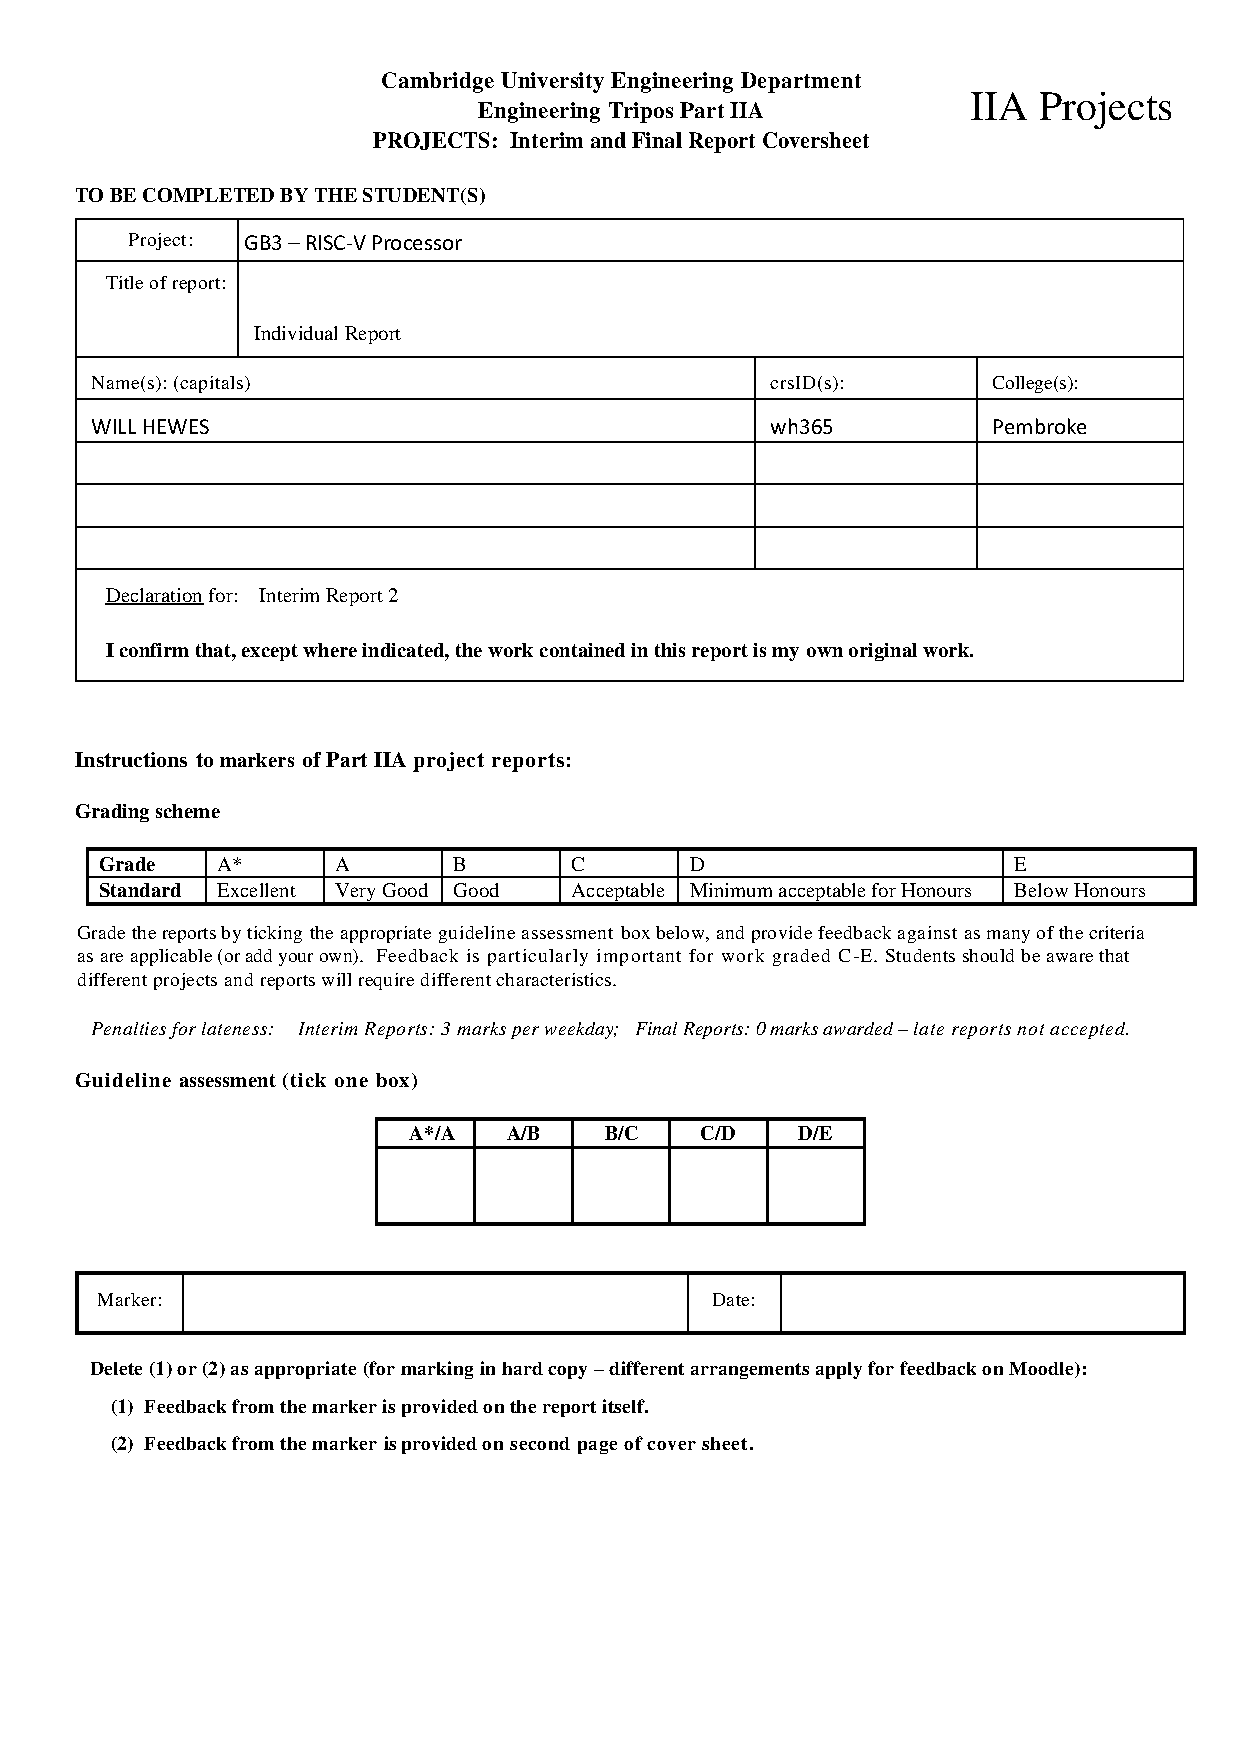
\includepdf[pages=-]{Handouts/IIA Project Coversheet Feedback Interim Report 2.pdf}
\maketitle
\hrule
\tableofcontents
\newpage

\section{Introduction}
\label{sec:Introduction}
% This section should give a detailed introduction to the changes
% you have implemented for your role on the team 
% (power/energy, time, or resource efficiency).

This report outlines the work carried out to reduce resource usage 
in the RISC-V processor implementation. 
My focus has been on optimising the Verilog modules 
most critical to logic utilisation, including the adder and program counter logic. 
The has has been to reduce the number of LUTs and flip-flops consumed
by the processor while minimising 
excessive power dissipation or performance degredation.
These modifications form part of a broader group effort targeting performance, 
power consumption, and resource usage. 
Coordination has been ongoing to ensure our changes are compatible and 
contribute towards a coherent final design.

The analysis has primarily been concerning the
\texttt{bubblesort} program due to its increased complexity,
allowing the processor to be pushed further and 
offering more representative resource utilisation patterns.
Preliminary synthesis results indicated that the original design 
made limited use of available DSP blocks, 
instead relying heavily on general-purpose LUTs for arithmetic operations.

To address this, the adder was restructured to map explicitly 
to the FPGA's DSP resources, freeing up LUTs and reducing logic congestion.
Additionally, the program counter logic was simplified 
by removing redundant operations and tightening the branching logic.
These changes collectively led to a reduction in logic cell usage, 
without strongly affecting other performance metrics.
Post-implementation metrics were captured using Yosys and nextpnr, 
with functional correctness verified via simulation against standard test programs.


\section{Preliminary Results}
\label{sec:Preliminary_Results}
% This section should provide detailed quantitative information and results so far.
\subsection{Baseline}
\label{sec:Baseline}

Having performed the baseline analysis in the previous interim report,
the resource usage for the provided processor on the \texttt{bubblesort}
algorithm is shown in table \ref{tab:baseline} the Appendix.

In the baseline design, 
synthesis of the unmodified processor design showed that approximately 
58\% of the available logic cells on the iCE40 UP5K were in use,
along with two third of the available Block RAMs. 
This figure indicates limited headroom for 
further feature integration or pipeline complexity, 
motivating efforts to streamline key datapaths and control logic. 
In particular, duplication in ALU operations, bloated forwarding logic, 
and unnecessary pipeline register toggling were identified 
as significant contributors to excessive logic usage. 
These observations guided the subsequent design changes detailed in this report.

\subsection{alu\_control.v}
\label{sec:alu_control.v}

The first module that was ammended was the ALU control module.
This is responsible for decoding instruction function codes into internal
ALU operation signals during operation.

The module initially had hardcoded ALU control values and function codes.
This had the consequence of duplicating logic for operations 
that were functionally equivalent but encoded separately. 
By replacing these constants with symbolic defines from 
\texttt{sail-core-defines.v}, 
the design now groups equivalent operations under shared identifiers, 
allowing the synthesiser to eliminate redundant logic paths. 
This change slightly reduces LUT usage without affecting functionality.

The results of this can be seen in table 
\ref{tab:bubblesort_pnr_report2} in the Appendix.
This resulted in a reduction of 7 LUTs compared to the baseline design.
While modest, this improvement contributes to the cumulative reduction 
in logic utilisation across the design and 
lays the groundwork for more impactful structural changes in downstream modules.

\subsection{alu.v}
\label{sec:alu.v}

\subsection{forwarding\_unit.v}
\label{sec:forwarding_unit.v}

\subsection{cpu.v \& pipeline\_registers.v}
\label{sec:cpu.v_and_pipeline_registers.v}

\section{Potential Risks}
\label{sec:Potential_Risks}
% This section should outline any challenges you ran into, 
% potential risks you see going into the final week, 
% and any steps you are taking to mitigate those risks.

\section{Future Work}
\label{sec:Future_Work}

\section{Conclusion}
\label{sec:Conclusion}

\newpage
\appendix
%Use this section to include diagrams, Verilog or C code, etc
\section{Resource Usage Data}

\begin{table}[H] 
    \centering
    \begin{tabularx}{0.6\textwidth}{X c c}
        \toprule
        Resource type & Used & \% of total \\ \midrule
        Logic cells (\texttt{ICESTORM\_LC}) & 3073 / 5280 & 58\,\% \\
        Block RAMs (\texttt{ICESTORM\_RAM}) & 20 / 30 & 66\,\% \\
        IO buffers (\texttt{SB\_IO}) & 8 / 96 & 8\,\% \\
        Global buffers (\texttt{SB\_GB}) & 5 / 8 & 62\,\% \\
        HF oscillators (\texttt{ICESTORM\_HFOSC}) & 1 / 1 & 100\,\% \\
        \bottomrule
    \end{tabularx}
    \caption{Baseline report}
    \label{tab:baseline}
\end{table}

\begin{table}[H] 
    \centering
    \begin{tabularx}{0.6\textwidth}{X c c}
        \toprule
        Resource type & Used & \% of total \\ \midrule
        Logic cells (\texttt{ICESTORM\_LC}) & 3073 / 5280 & 58\,\% \\
        Block RAMs (\texttt{ICESTORM\_RAM}) & 20 / 30 & 66\,\% \\
        IO buffers (\texttt{SB\_IO}) & 8 / 96 & 8\,\% \\
        Global buffers (\texttt{SB\_GB}) & 5 / 8 & 62\,\% \\
        HF oscillators (\texttt{ICESTORM\_HFOSC}) & 1 / 1 & 100\,\% \\
        \bottomrule
    \end{tabularx}
    \caption{Report after ... make to ...}
    \label{tab:bubblesort_pnr_report2}
\end{table}

\section{Code}

\section{Interim Report 1}
\label{sec:{Interim_Report_1}}
\includepdf[pages=3-]{Reports/wh365-interim-report-1.pdf}

\end{document}